
%(BEGIN_QUESTION)
% Copyright 2006, Tony R. Kuphaldt, released under the Creative Commons Attribution License (v 1.0)
% This means you may do almost anything with this work of mine, so long as you give me proper credit

A very common method for controlling the ``flow'' of a powdered or granular solid into a process is a variable-speed conveyor belt and scale mechanism called a {\it weighfeeder}, or {\it gravimetric belt feeder}.  One possible application for a device like this is metering powdered coal into a furnace or a large power-generation steam boiler:

$$\includegraphics[width=15.5cm]{i01431x01.eps}$$

In the above illustration, a short section of the belt is supported by a set of rollers connected to a load cell.  This effectively weighs a section of the loaded belt.  If we know how long that section of rollers is, the weight indication in pounds can be translated into a figure of pounds per foot (of belt).  All we need to know is the belt speed and we can figure pounds per minute of material delivered to the process.

Explain how a variable-speed electric motor is essential for being able to control the amount of solid material going to the process.  Also identify what devices would need to be {\it locked out} for safety before any mechanical maintenance work was done to the system.

\vskip 20pt \vbox{\hrule \hbox{\strut \vrule{} {\bf Suggestions for Socratic discussion} \vrule} \hrule}

\begin{itemize}
\item{} If you were tasked with programming a PLC to calculate real-time mass flow rate over this weighfeeder, how would you do it (in general terms)?  What sensors would you need to install?  How many analog input channels would your PLC need to have?  What sort of calculation(s) would the PLC need to do on the signals?
\end{itemize}

\underbar{file i01431}
%(END_QUESTION)





%(BEGIN_ANSWER)

Usually, the belt's drive motor is variable-speed, as well as the motor driving the rotary feeder.

%(END_ANSWER)





%(BEGIN_NOTES)

%INDEX% Final Control Elements, motor: weighfeeder

%(END_NOTES)


